\chapter{Hash Function \& MAC}

\begin{flushleft}
    Abbiamo visto che le configurazioni di sicurezza della crittografia simmetrica sono: \textbf{confidenzialità}, \textbf{integrità} e \textbf{autenticità}. Abbiamo anche definito che Alice e Bob condividono la conoscenza di un'unica chiave per la comunicazione. Con i \textit{block cipher} siamo riusciti a ottenere \textbf{confidenzialità}. 

    \medskip

    \textcolor{red}{\textbf{\textit{Integrity}}}: è possibili identificare dal ricevente di un messaggio se quel messaggio è stato modificato durante la trasmissione. Consideriamo una comunicazione tra Alice e Bob, dove il messaggio verrà inviato da Alice, prima di farlo verrà calcolato a \textbf{\textit{small-sized digest}} che rappresenta il dato. In questo modo qualunque modifica al dato o al \textbf{\textit{digest}} può essere verificata - in questo caso non c'è bisogno della chiave - $d = H(m)$ dove:
    \begin{itemize}[nosep]
        \item \textbf{d} è il \textit{digest} della funzione.
        \item \textbf{H} è una funziona che ritorna una sequenza di byte che rappresenta il dato.
        \item \textbf{m} è il messaggio.
    \end{itemize}
    Alice a quel punto invia a Bob $m || d$ in questo modo, Bob può ricalcolarsi $d' = H(m)$ e accettare il messaggio da Alice - quindi verificarne l'\textbf{integrità} - se e solo se $d == d'$.

    \medskip

    \textcolor{red}{\textbf{\textit{Authenticity Guarantess}}}: il destinatario del messaggio può controllare se il mittente è un mittente legittimo - ovvero qualcuno che ha accesso alla chiave segreta simmetrica - è possibile \textit{bindare} una qualche informazione (metadato) per rendere l'informazione identificativa, ma quasto è utile solamente nella crittografia asimmetrica.

    \begin{figure}[h]
        \centering
        \includegraphics[width=0.55\textwidth]{img/mac_tag.png}
    \end{figure}

    L'integrità dell'informazione è condizione necessaria per l'autenticità, se l'attaccante può modificare il dato, allora può anche impersonificare il mittente del dato, violando l'autenticità.

    \smallskip

    È spesso confusa l'integrità del dato con la sua autenticità, nel contesto della sicurezza informatica noi cerchiamo l'autenticità - e quindi implicitamente l'integrità - per questo motivo andremo ad analizzare \textbf{\textit{authenticated encryption}}. È però fondamentale differenziare le due proprietà in quanto utilizzano schemi di crittografia differenti:
    \begin{itemize}[nosep]
        \item \textbf{\textit{Integrity}} utilizzo delle \textbf{funzioni hash}.
        \item \textbf{\textit{Authenticity}} utilizza i \textbf{\textit{Message Authentication Code - MAC}}, per ora andremo ad analizzarli nell'ambito della crittografia simmetrica.
    \end{itemize}

    \textcolor{red}{\textbf{\textit{Hash function \& cryptographic integrity guarantees}}} \\
    Andiamo, velocemente, ad analizzare quelle situazioni in cui è richiesta \textbf{\textit{integrità}} fuori dai requisiti di crittografia: come ad esempio modifiche al dato per errori di trasmissione o per guasti - normalmente scaturite da fenomeni fisici - per i quali sono presenti molteplici algoritmi, tra i quali: \textbf{\textit{parity}}, \textbf{CRC}, \textbf{\textit{checksum}}. In questo caso è possibile modellare la tipologia di attaccante come un \textbf{attaccante irrazionale} (perdita di bit randomici o a raffica). \\
    Nei settaggi di crittografia moderna, l'attaccante è sempre \textbf{razionale} e conosce gli \textbf{algoritmi crittografici} e si comporta di conseguenza, grazie al requisito di \textbf{\textit{cryptographic integrity-protection}} anche se noti i dati di base non deve essere capace di trovare una soluzione al problema nonostante l'assenza di una chiave condivisa. Anche in questo caso è presente la sicurezza computazione ma viene applicata in maniera differente.

    \medskip

    \textcolor{red}{\textbf{Cryptography Hash Function}}: una funzione hash $H$ viene definita come: 

    {\centering
        $H : \{0, 1\}^* \mapsto \{0, 1\}^n$
    \par}

    ovvero è possibile mappare una quantità arbitraria di bit - nelle moderne funzioni hash $*$ è così ampio che può anche considerato a $\infty$ - in una sequenza fissata (piccola) - che è definita dall'algoritmo. L'ouput di $H$ viene chiamato \textbf{\textit{digest}} - le funzioni di hash esistono anche per scopi non prettamente crittografici. La dimensione di \textbf{n} è scelta in maniera tale che sia altamente improbabile che due input differenti generino lo stesso output, in questo modo il \textit{digest} è un informazione ``piccola'' che rappresenta univocamente l'informazione contenuto nel dato. È possibile paragonare il comportamento ad una \textbf{funzione di compressione pseudorandom}

    {\centering
        $m_1 \neq m_2 \longleftrightarrow d_1 \neq d_2$
    \par}

    Il comportamente delle funzioni hash - \textbf{PRF} - può essere applicato anche a circostante non crittografiche, ad esempio: \textbf{MD5} è una funzione hash deprecata, ma viene utilizzata per identificare in maniera univoca i commit su git. È possibile anche utilizzarle come \textbf{primitive} per costruire blocchi per altri schemi crittografici, ad esempio: alcuni \textbf{MAC} si basano su delle \textit{hash function} ed anche alcune \textbf{\textit{Key Derivation Function - KDF}}.

    \medskip

    In base al tipo di applicazione che stiamo utilizzando bisogna che la funzione hash sia resistente a diversi \textbf{\textit{attack model}}, tutti quanti, se no viene definita \textbf{deprecata}.

    \textcolor{red}{\textbf{\textit{Attack Models} Differenti}}
    \begin{center}
        \begin{minipage}[c]{0.75\textwidth}
            \begin{itemize}[nosep]
                \item \textbf{\textit{One Way}} anche nota come \textbf{\textit{first pre-image resistance}}, deve essere \textbf{efficiente} calcolare $H(m) = d$, ma \textbf{inefficiente} calcolare la funzione opposta, ovvero risalire a $m = H^{-1}(d)$
                \item \textbf{\textit{Second pre-image Collision Resistant}} ovvero dato un messaggio $m_1$ è \textbf{inefficiente} trovare un messaggio $m_2$ tale che $H(m_1) = H(m_2)$
                \item \textbf{\textit{Collision Resistant}} è \textbf{inefficiente} trovare una coppia di messaggi - \textbf{arbitrari} - $m_1$ e $m_2$ tale che $H(m_1) = H(m_2)$
            \end{itemize}
        \end{minipage}
        \hfill
        \begin{minipage}[c]{0.1\textwidth}
            \centering
            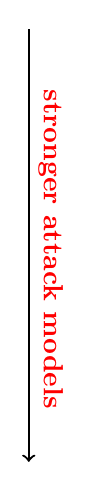
\begin{tikzpicture}[scale=1]
                \node[rotate=270, anchor=south, text=red] at (0,2.2) {\textbf{stronger attack models}};
                \draw[<-, thick, black] (0,-0.5) -- (0,5.0);
            \end{tikzpicture}
        \end{minipage}
    \end{center}

    \textcolor{red}{\textbf{\textit{First pre-Image Resistance}}}: dato un \textit{digest}, calcolarsi il dato. È tipicamente associato a \textbf{garanzie di confidenzialità} - può essere applicato a schemi di \textbf{KDF}.

    \begin{figure}[h]
        \centering
        \includegraphics[width=0.45\textwidth]{img/one_way.png}
    \end{figure}
    
    Dato in input una chiave, ottengo in output un'altra chiave $k' = H(k)$ in questo caso cosa dovrebbe rompere Eve per riuscire a decifrare? In questo contesto anche se $H$ \textbf{non} è \textit{collision resistance} non è di interesse infatti anche se si trovasse un $k'' \; \text{t.c.} \; k' = H(k'') \rightarrow k \neq k''$ e quindi Eve non riuscirebbe a rompere lo schema crittografico di cifratura, l'unico modo per Eve di ottenere il dato in chiaro è riuscire a trovare una funzione $H^{-1} \; \text{t.c.} \; k = H^{-1}(k')$ e utilizzarla per decifrare le informazioni di Alice - ci basta: \textbf{\textit{One Way}}. \\
    L'unica limitazione è che se l'input $k$ è debole e quindi vulnerabile a \textit{brute-force} allora sarebbe possibile eseguire una ricerca esaustiva nell'insieme delle chiavi - \textbf{\textit{HKDF}}.

    \medskip

    \textcolor{red}{\textbf{\textit{Second pre-Image Collision Resistance}}}: dato un $d$ e un $m$ tale che $d = H(m)$ trovare un valore $m' \; \text{t.c.} \; d = H(m')$ è tecnicamente richiesta per gli \textbf{\textit{authentication schemes}} ad esempio nel contesto di \textbf{\textit{Keyed Hash Function}} - per l'offuscamento di password su DB - infatti riuscendo o a trovare $H^{-1}$ o trovando un'altro valore $m'$ che generi lo stesso \textit{digest} è possibile bypassare il controllo.
\end{flushleft}

\begin{boxA}
    \textcolor{orange}{\textbf{Esempio}}: \textbf{Download di dati}

    \medskip

    {\centering
        \includegraphics[width=0.45\textwidth]{img/hash_es.png}
    \par}

    Quando un sito mette a disposizione dei dati per il download - ad esempio un \textit{*.iso}, normalmente il contenuto per il download è disponibile su un \textit{server mirror}, quindi il \textit{provider} si calcola il \textit{digest} $d = H(m)$ e poi fa l'upload del contenuto sul \textit{server mirror}. L'utente si scarica il contenuto dal \textit{server mirror} e scarica il \textit{digest} dal \textit{provider}, successivamente calcola l'hash del dato scaricato $d_u = H(m_d)$ se e solo se $d_u = d$ accetta il dato scaricato.

    \smallskip

    In questo caso la funzione hash $H$ deve rispettare la ``normativa'' di sicurezza \textit{second pre-image collision resistance} in quanto il messaggio iniziale - la nostra \textit{*.iso} - viene fornita dal provider. L'attaccante vincerebbe se riuscisse a trovare un messaggio $m_a \; \text{t.c.} \; H(m_d) = H(m_a)$ e contemporaneamente quel messaggio dovrebbe contenere un \textit{payload} malevolo. Solo in quel caso l'utente lo scaricherebbe il messaggio e la funzione di verifica - chiamata \textbf{\textit{verify}} - andrebbe a buon fine e quindi l'utente accetterebbe il nuovo messaggio.
\end{boxA}

\begin{flushleft}
    \textcolor{red}{\textbf{\textit{Collision Resistance}}}: riuscire ad ottenere, arbitrariamente, due messaggi $m_1$ e $m_2$ tali che $H(m_1) = H(m_2)$ è la più forte come garanzia di sicurezza, nel caso dovesse mancare, la funzione hash sarebbe molto facile da violare.
\end{flushleft}